\section{Key Network Parameters and Derived Cost Functions}
\label{ch1:sec:key-network-parameters}

In literature (see Chapter \ref{ch-review}), two distinct approaches have been used to improve performance of a system.
Either cost is reduced or utility is maximised.
Both approaches rely on a mathematical explanation of the underlying features that relate to performance of the system.
To reiterate, utility ought to be maximised, since the benefit of the underlying mechanisms ought to be increased to a maximum, whereas cost should be minimised.
The choice for this piece of work was to relate key network parameters to associated cost functions, with the reason that a cost can be minimised to a finite value of zero.
This means that solutions to a cost function, where the resulting cost is zero, are by definition optimal solutions, whereas a utility function can have multiple maxima that need not be the best solution.
To illustrate this feature, an arbitrary utility function, $\zeta^{*}(x)$, and cost function, $\zeta(x)$, have been plotted in Figures \ref{ch1:subfig:sketch-utility} and \ref{ch1:subfig:sketch-cost}, respectively.

\begin{figure}\centering
	\subfloat[Sample utility function]{%
		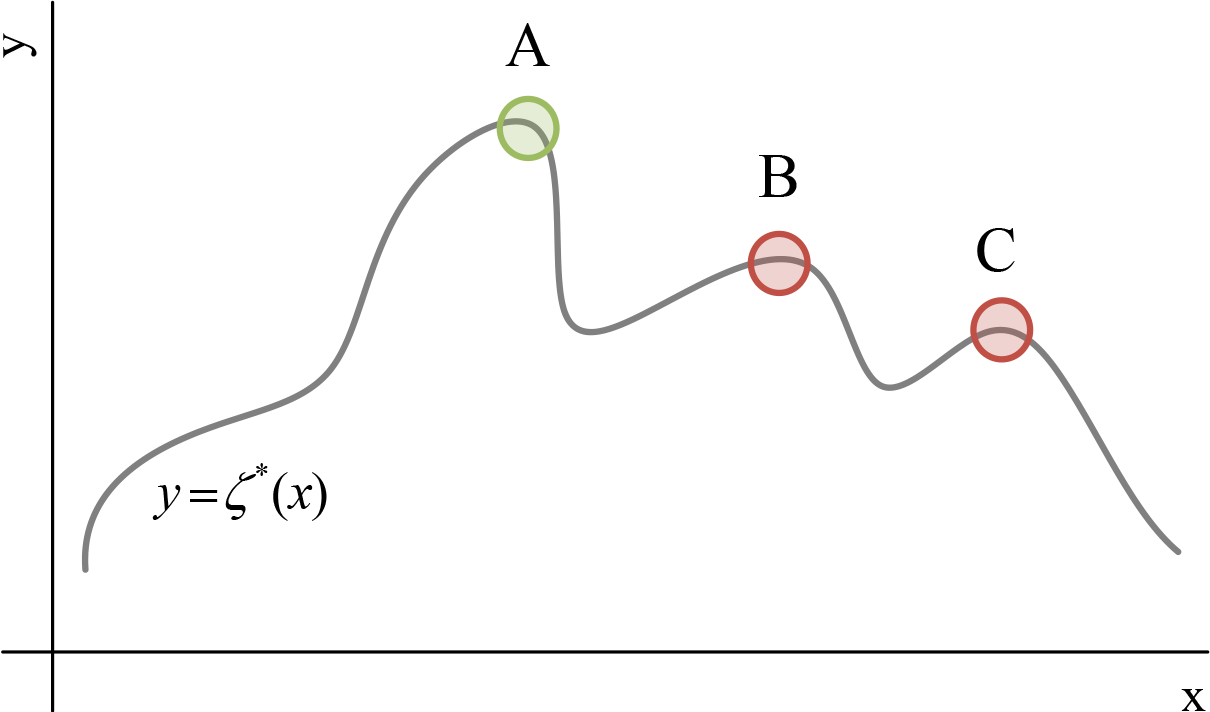
\includegraphics[width=0.45\textwidth]{_chapter1/fig/sketch-utility}%
		\label{ch1:subfig:sketch-utility}%
		}
	\hspace{5mm}
	\subfloat[Sample cost function]{%
		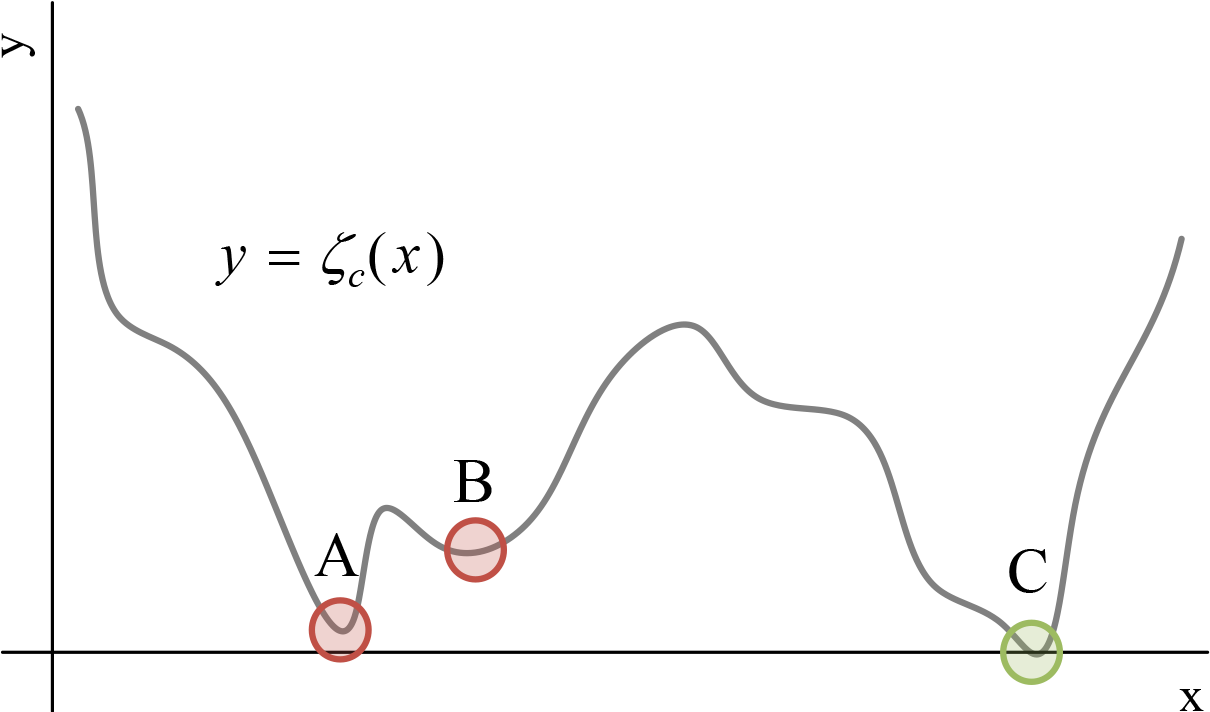
\includegraphics[width=0.45\textwidth]{_chapter1/fig/sketch-cost}%
		\label{ch1:subfig:sketch-cost}%
		}
	\caption{Benefit of using cost function over utility function}
	\label{ch1:fig:sketch-utility-vs-cost}
\end{figure}

Again, these two figures illustrate how the peaks of the utility function are at different, large values of $y$, whereas the troughs of the cost function always approach zero.
Depending on the starting condition, i.e. the initial values for $x$, different maxima or minima (i.e. points $A$, $B$ or $C$) may be found.
Here, the best solution for $\zeta^{*}(x)$ is at point $A$, whereas the best solution for $\zeta(x)$ is at point $C$.
Whilst point $A$ represents the highest utility, it does not imply optimum system performance, as utility is unbounded, i.e. $\zeta^{*}(x) \in (-\infty, \infty) \forall x$.
In contrast, for the cost function, point $C$ would represent an absolute minimum, since a cost function's range is greater or equal to zero, i.e. $\zeta(x) \geq 0 \forall x$.
Therefore, the cost's proximity to zero directly indicates the system performance (whilst the utility's proximity to infinity would not make sense).

With this in mind, the key network parameters can be explained and the corresponding cost functions can be defined.
The choice of parameters is virtually inexhaustible since one could treat every single current, voltage or phase angle as a potential network parameter.
In reality (particularly in the context of NTVV), a power distribution network could only be probed at two points: the substation and the ESMU.
Therefore, all these possible measurements and the derived parameters are treated as key network parameters; these parameters are from hereon referred to as ``realistic parameters''.
For the work presented in this chapter, all realistic parameters are extracted from power flow simulations.

In this simulation of a power distribution network (i.e. in OpenDSS), a system of nodal power flow equations is solved.
In the IEEE LV Test Case, there are 906 three phase buses, resulting in 2718 nodes for which current and voltage can be obtained.
This abundance of values means that a lot of additional parameters, that could not easily be measured in reality may also be included in the set of key network parameters; these parameters are from hereon referred to as ``theoretical parameters''.
To restrict the amount of theoretical parameters, they were chosen based on their importance and impact on actual network operation.

A list of both realistic and theoretical key network parameters\footnote{A key network parameter is marked with a dagger ($\dagger$) if it is a theoretical parameter that can only be extracted form the power flow simulation.} is presented below, before going into detail for each parameter:

\begin{itemize}
	\item Voltages at substation transformer's secondary winding
	\item Voltages at ESMU's PCC
	\item Voltages at customer lateral$^{\dagger}$
	\item Total power flow
	\item Line utilisation
	\item Distribution losses$^{\dagger}$
\end{itemize}

\subsection{Voltages at substation}
\label{ch1:subsec:voltages-at-substation}

In UK LV distribution networks, the substations supply power to the feeding cable.
Substations provide the link from MV distribution network, which operates at 11kV P2P, to the LV distribution network, which operates at 230V P2N (i.e. 400V P2P).
If the substation transformer was an ideal transformer, then the voltage measured at its secondary winding would remain constant.
In reality however, the internal losses (e.g. conductive losses and magnetic leakage) lead to a drop in voltage with increasing load.
Therefore, any deviation from the substation's nominal voltage may be a result of suboptimal network operation.

If one defines the substation voltage as a single phase voltage $v_{ss,p}(t)$, where $p$ is the phase number and $t$ the time at which the measurement was taken, then a divergence cost can be calculated as $\zeta_\text{substation voltage}(v_{ss,p}(t)) \forall t$.
This cost is defined as:

\begin{equation}
	\zeta_\text{substation voltage}(v_{p}) := \sum_{p=1}^{3}{\begin{cases}
		\zeta_h(v_p) & \text{if } V_{ss} \leq v_p\\
		\zeta_l(v_p) & \text{otherwise}\\
	\end{cases}}
	\label{ch1:equ:substation-voltage-deviation}
\end{equation}

Here, $\zeta_h(v)$ and $\zeta_l(v)$ are functions that convert the single phase voltage $v_p$ into a normalised and increasing, positive cost.
If the voltage $v_p$ is greater than or equal to the nominal substation voltage $V_{ss}$, then the result from $\zeta_h(v)$ is used, otherwise the result from $\zeta_l(v)$ is used.
To define these two functions, the nominal voltage $V_n$, of 230V P2N, and the corresponding high and low voltage thresholds, $V_h$ and $V_l$ respectively, need to be introduced.

\begin{equation}
	\zeta_h(v) := \left|\left(\frac{v-V_{ss}}{V_h-V_n}\right)^2-1\right|^{-1}
	\label{ch:equ:high-voltage-threshold-cost}
\end{equation}

\begin{equation}
	\zeta_l(v) := \left|\left(\frac{V_{ss}-v}{V_n-V_l}\right)^2-1\right|^{-1}
	\label{ch:equ:low-voltage-threshold-cost}
\end{equation}
a
\subsection{Voltages at ESMU's PCC}
\label{ch1:subsec:voltages-at-esmu}



\subsection{Voltages at customer laterals}
\label{ch1:subsec:voltages-at-customers}



\subsection{Total power flow}
\label{ch1:subsec:total-power-flow}



\subsection{Line utilisation}
\label{ch1:subsec:line-utilisation}



\subsection{Distribution losses}
\label{ch1:subsec:losses}





